%todo = interact to interaction in fig 6.4
\documentclass{cslthse-msc}
\usepackage[utf8]{inputenc}
\usepackage[english]{babel}
\usepackage{amsmath}
\usepackage{amsfonts}
\usepackage{amssymb}
\usepackage{amsthm}
\usepackage{graphicx}
\usepackage{tikz}

%\bibliographystyle{alpha}

\usepackage[titletoc, header, page]{appendix}
\usepackage{verbatim}
\usepackage{chronology}


\usepackage{hyperref}

\author{
	Jens Gustafsson \\
	{\normalsize \href{mailto:ada10jgu@student.lu.se}{\texttt{ada10jgu@student.lu.se}}}
	\and
	Alfred Åkesson \\
    {\normalsize \href{mailto:ada10aak@student.lu.se}{\texttt{ada10aak@student.lu.se}}}
}

\title{Formatting a Master's Thesis}
\subtitle{A {\LaTeX} class}
%\company{The Corporation AB LTD Inc}
\supervisors{John Deer, \href{mailto:jdeer@company.com}{\texttt{jdeer@company.com}}}{Don Jeer, \href{mailto:djeer@xy.lth.se}{\texttt{djeer@xy.lth.se}}}
%\supervisor{John Deer, \href{mailto:jdeer@company.com}{\texttt{jdeer@company.com}}}
\examiner{Jane Doe, \href{mailto:jane.doe@cs.lth.se}{\texttt{jane.doe@cs.lth.se}}}

\date{\today}
%\date{January 16, 2015}

\acknowledgements{
If you want to thank people, do it here, on a separate right-hand page. Both the U.S. \textit{acknowledgments} and the British \textit{acknowledgements} spellings are acceptable.

We would like to thank Lennart Andersson for his feedback on this template.
}

\theabstract{
This document describes the Master's Thesis format for the theses carried out at 
the Department of Computer Science, Lund University. 

Your abstract should capture, in English, the whole thesis with focus on the problem and solution in 150 words. It should be placed on a separate right-hand page, with an additional \textit{1cm} margin on both left and right. Avoid acronyms, footnotes, and references in the abstract if possible.

Leave a \textit{2cm} vertical space after the abstract and provide a few keywords relevant for your report. Use five to six words, of which at most two should be from the title.
}

\keywords{MSc, template, report, style, structure}

%% Only used to display font sizes
\makeatletter
\newcommand\thefontsize[1]{{#1 \f@size pt\par}}
\makeatother
%%%%%%%%%%


\begin{document}
\makefrontmatter


\chapter[Introduction]{Introduction}
%in need of a kidney transplant can not undergo surgery

Many people suffering from renal failure are in need of a kidney transplant. A problem in the health care is that patients can not undergo surgery if they have too much belly fat. It is very hard for this group of people to loose weight, as further described in section \ref{sec:kiney}. Regular exercises and physical activities are therefore something crucial for this group of people. A project group at the Skåne University Hospital has recently been established to help this group of people to loose weight. A question they asked themselves was whether it was possible to use any activity tracking devices in this project.

Sony has developed wearable devices that can track a user’s daily activities. The data collected by these devices are saved online in their database and accessible through an API called the LifeLog API. Sony wants to investigate what different use cases that exists for their wearable devices and has therefore chosen to sponsor this project with smart wristbands for the patients to wear.

itACiH is a research project that is investigating the possibilities of advanced health care at home. As a part of this project a planning-system was developed that currently is in use at the hospital. This planning system is built as a web application. The system is built such that it remotely can fetch data from sensors that are installed at the home of a patient. Because itACiH is already in use at hospital the system developed in this thesis will use the same platform as itACiH for easy later integration at the hospital. 

This thesis presents a system that aims to help over-weight patients with renal failure to loose weight. The system is called the Region Skåne Activity tracking, or the RSAT for short. The project group will be called the RSAT-group in this thesis.




\newpage

\section{Purpose and question formulation}

The purpose of this thesis is to build a system that can be used in the health care to help patients with kidney failure to loose weight. The Sony Lifelog API will be used as the foundation for the system. As a step in building the system, an investigation about how well suited the API is to be used will also be performed. 



A technical evaluation of SONY Lifelog API for use in heath care.

How good is SONY Lifelog  for use in heath care from a technical standpoint?

How good is RSAT?

\begin{comment}
The following questions will be used to fulfill the purpose: 

\begin{quote}
\centering
\emph{In what ways can the Sony Lifelog technology be used in the health care to help patients with renal failure?}
\end{quote}


This is a very broad question, and it has therefore been divided into three sub questions:

\begin{enumerate}
    \item \emph{What other platforms exists on the market that could have been used instead of the Sony Lifelog?}
    \item \emph{What are the pros and cons of using the Sony Lifelog API?}
    %\item \emph{}
    %\item \emph{What data in the Lifelog API is useful for the health care?}
    %\item \emph{What functionality does not exist in the Sony Lifelog technique which would be useful for the health care?}
    \item \emph{What problems, if any, do arise when third party API:s are integrated in the health care, from a technical standpoint?}
\end{enumerate}

The system will be made up from requirements that have been created in collaboration with a physiotherapist. The physiotherapist is working with patients suffering from chronic kidney disease on a daily basis and is the one who will be using the system. These requirements will be presented in \ref{sec:req}. 

\end{comment}
\section{Method}%TODO

The method used for the development of the system was by first talking to the RSAT-grope and listen to there wishes. Then making a prof of concept solution to get familiar with the API. By using the experience of from the development of the prof of concept requirements was formed together with the RSAT-group. The approach for the development was to use iterations. Each iteration resulted in a demo for the RSAT-group. During the demo feedback was given from the RSAT-group. The experience from the development of the system lay down the ground for the evaluation of both Lifelog and RSAT.






%As the purpose of this thesis is twofold; (1) to investigate in what ways the Sony Lifelog API is useful in the health care and, (2) to build an actual system based on the API, the work carried out in this thesis is divided into three main parts, one research part, one development part and one evaluation part. 

% This thesis is divided into three main parts; one research part, one development part and one evaluation part. In the research part facts about other systems similar to the one to be built will be gathered. Information about other activity trackers will also be collected in order to evaluate the Sony Lifelog and to compare it with other platforms. In the development, the development of the system will be performed and explained. In the evaluation part the RSAT will be evaluated and compared to other existing systems. The Sony Lifelog API will also be evaluated and compared to other API:s.  

% During the project, three different prototypes will be built and the development cycle of each prototype will consist of the following steps:

\begin{enumerate}
\item Identify the requirements for the current prototype
\item Implement functionality in the system such that the system fulfills the requirements.
\item Test the developed prototype and publish it such that others can test our software.
\item Receive feedback from testers and use it as input to the next prototype. 
\item Receive new requirements on the system, if the requirements are feasible, add them to a later iteration. 
\end{enumerate}

%%%%%%%%%%%%%%%%%%

\section{Disposition}

The fist part of this thesis gives an overview of the landscape that RSAT acts in. Fist a medical background is given. Then a technical background describing the techniques used in RSAT. After that works related to the thesis is described. First different warble technologies and platforms for aggregation of activity data and  systems similar to RSAT. 

The second part contains a description of the development of RSAT. From the initial thoughts in the RSAT group to the last prototype. Telling about all decision and struggles.  

At last the RSAT and Lifelog is evaluated and compared to other systems described in the first part of the thesis.

%Third part evaluate both Lifelog and RSAT by comparing them to solutions and standards described in the first part of the thesis.

%In the first part, an overview of the current state of the art of wearable technology is given. Also different platforms that can be used to aggregate health data are presented. In the second part, an actual system is developed. At last the system is evaluated and compared to other systems. %TODO


% BRA KÄLLA to be used: http://www.kidney.ca/facing-the-facts

\chapter{About chronic kidney disease}

The kidneys have the responsibility of filtering waste products from the blood in the body\cite{NKDEPBASICS}. When the kidney function is too low to filter the blood, dialysis and in the end a kidney transplant, is needed.

In this chapter an introduction to chronic kidney disease is given. The following chapter begins with a short introduction to chronic conditions in general. Chapter 2.2 discusses chronic kidney disease especially.  

\section{Chronic conditions}

%Treating chronic condition is a huge part of the health care, especially in the western world. 

% todo: kan man skriva "go to treating" är go to kanske lite "sv-engelskt"? Tror klar hittar du fel jens fixa.

The costs in the health care are ever increasing. A huge part of the health care and the economic costs associated with it addresses patients with chronic conditions. More than 60\% of all deaths in the world is due to this types of complications. In Sweden 80\% of all the health care costs go to treating these conditions\cite{SmartCare}. A study shows that three types of lifestyle behaviors leads to four chronic diseases. These diseases accounts for about 50\% of all the deaths worldwide, see figure \ref{fig:chronic-fig}\cite{callaway2015quantified}. 

\begin{figure}[!hbt]
\centering
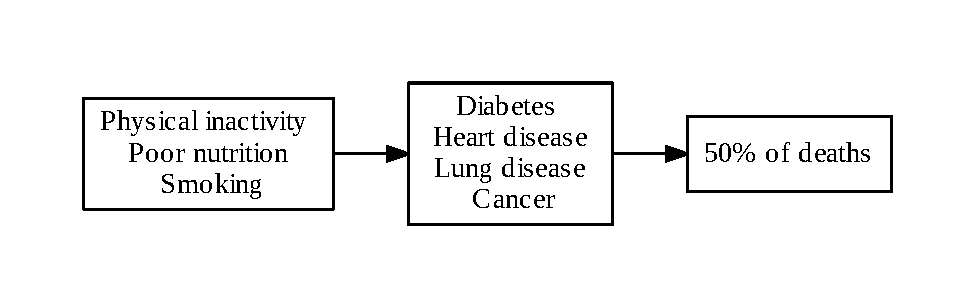
\includegraphics[scale=0.8]{chronic-fig.pdf} 
\caption{Figure  describing what lifestyle behaviors that increases the risk of death}\label{fig:chronic-fig}
\end{figure}

As seen in figure \ref{fig:chronic-fig} physical inactivity is one factor that could lead to a chronic condition. 

%There are also other chronic condition that will benefit from physical activity and more information about one of them in the section below. 

%% Den utmarkerade texten ovan kanske ska mergeas, läggas till igen på något vis när kidney failure-sektionen är genomgången. 

\section{Chronic kidney disease}
\label{sec:kiney}
\begin{comment}
NKDEPBASICS: http://nkdep.nih.gov/learn/kidney-disease-basics.shtml
KIDNEYFOUNDATION: https://www.kidney.org/kidneydisease/aboutckd
NKDEPPROG: http://nkdep.nih.gov/identify-manage/manage-patients/slow-progression.shtml
DIALYSIS: http://www.vardhandboken.se/Texter/Dialys-peritonealdialys/Oversikt/
\end{comment}

Chronic kidney disease (CKD) is a gradual loss of kidney function over time\cite{KIDNEYFOUNDATION}. There are no specific symptoms of the disease but illness, tiredness and a reduced appetite are all common symptoms. As the kidney function is worsening, waste products builds to high levels in the blood that may cause complications such as high blood pressure,  muscle- and bone mass loss. The risk of getting other diseases such as cardiovascular disease, ericarditis and anemia is also growing.  When the waste products in a patient’s body becomes so high that the patient starts to get sick from it, the patient requires dialysis\cite{KIDNEYFOUNDATION}.

People with severe CKD are in need of a kidney transplant. Until a transplant can be performed, dialysis is required. Without dialysis, the patients would have a poor life expectancy\cite{KIDNEYFOUNDATION}. Dialysis is a cumbersome treatment process for a patient as it takes up a lot of time and adds a lot of constraints to the patient’s life. Dialysis is also expensive for the society. A rough estimate of the yearly cost of treating one patient with dialysis in Sweden is 500 000 – 1 000 000 SEK. 

Peritoneal dialysis and hemodialysis are dialysis that can be performed in the home of a CKD-patient. The principle behind peritoneal dialysis is that a sterile solution containing glucose is run in to the patient’s abdomen\cite{DIALYSIS}. The peritoneum inside the patient acts as a membrane across which waste products from the blood is filtered. A downside with the peritoneal dialysis is that the calorie intake increases, since the sterile solution contains glucose. Hemodialysis is a kind of blood dialysis, where blood is filtered outside the body.

Despite that CKD is considered to be an irreversible condition, the progress of the disease can be slowed down. The National Kidney Disease Education Program (NKDEP) lists three strategies that can be used to slow down the progress\cite{NKDEPPROG}. One of those strategies is lifestyle interventions and addresses different health-promoting behaviors. One of the health-promoting behaviors they discuss is physical activity. NKDEP states that people suffering from CKD has the same recommendations for physical activity as the general population. 

Eventually, a patient with CKD must undergo a kidney transplant. The patient must be in good physical shape, as the risk of infections and other diseases otherwise are too high. It is also essential that the patient does not have to much belly fat. Not only does the fat induce a greater risk for the patient's life, it also makes it harder for surgeons to practically perform the transplant. Vad kostar det?!
%http://www.kidney.ca/document.doc?id=4083
%http://health.costhelper.com/kidney-cancer.html

\chapter[Technical Background]{Technical Background}

This chapter describes the techniques used to develop RSAT. First Sony Lifelog and techniques used by Lifelog described.The second part of the describes Palcom the platform used by the itACiHi and RSAT. 

\section{Sony Lifelog}

% Write about the smart armband
The Sony Lifelog application is an Android application which is built around the idea about logging a users lifestyle and daily activities\cite{LifeLogDescr}. The application collects various data about its users through different sensors in a smartphone and SmartWear-devices (Sony SmartWatch or a Sony Smartband) and displays it to the user. Example of data it logs are information about what applications in the smartphone that have been used, what locations that have been visited and information about different physical activities performed during the day.  

\subsection{Sony SmartBand}

The Sony SmartBand SWR10 is the chosen wristband for this project. The Sony SWR10 has a movement sensor which recognizes different movements a user is doing\cite{SWR10}. This data is analyzed by Sony and categorized into different activites which are uploaded to a central repository that stores the data. The SmartBand must be connected to an Android device with Android version 4.4 or higher to be able to collect data. 

\subsection{The Sony Lifelog API} 
All the data collected in the Sony Lifelog application are automatically uploaded to a central repository that stores the data. This data is globally accessible through a REST-based web-serviceAPI\cite{LifeLogDescr}. 

The API has three different endpoints; a profile endpoint, an activities endpoint and a location endpoint. The profile endpoint contains basic information about a user's name, age, height and weight and is entered by the user into the Lifelog application. The activities endpoint contains the different data Lifelog has logged about performed activities throughout the day such as physical activity. All activities has a type and some also has a subtype. 

%Examples of data a user can log is data about her sleep or how many steps she has walked during the day. 
The location endpoint provides a list of coordinates specifying what locations a user has been visiting during a time period. Activities and locations in the API are associated with times. A response from the API always includes the time stamp of the earliest and latest included entry. The format of the timestamp follows the ISO 8601 standard. 

The API can be accessed by third parties to retrieve collected data about a user. Every request made to the API must be authorized and https must be the chosen communication protocol. The lifelog Web API uses OAuth 2.0 as its authorization mechanism. To connect to the API, a user must login and give explicit permission for the application or the service to access to the data. 

The response to a valid request made to the API contains a result-section. This result-section is a set of data represented as json objects. If the requested data is to large to fit in the size of one response message, the data is split up into several messages and a link-field is inserted into the response. This link-field contains a link pointing to the location from where the rest of the data can be fetched. 




%%%%%%%%%%%%%%%%%%%%%%%%%%%%%%%%%%%%%%%%%%%%%%%%%%%
\begin{comment}
The response can also contain an error message:
403 AccessDenied				you do not have permission to access
401 InsufficientAuthentication	No access token or an invalid access token was sent in the request
404 ResourceNotFound			The data does not exist
422 UnprocessableEntity 		Request could not be parsed or contained invalid values
\end{comment}

%%%%%%%%%%%%%%%%%%%%%%%%%%%%%%%%%%%%%%%%%%%%%%%%%%


\subsubsection{REST}
\label{sec:rest}

The Sony Lifelog API is a REST API. REST is an architectural style for designing API:s and are heavily used in modern web services. The concept is to represent resources as the analogy for the data endpoints and to have a small set of actions interacting with these resources. The REST architectural style has the following principles\cite{pautasso2014restful}:

\begin{itemize}
    \item \emph{Addressabilty} All resources must be addressable with a unique identification. On the web each resource uses a unique URI such that it becomes globally addressable.
    \item \emph{Uniform Interface} The interface to the resources should according to REST be uniformed and simple. On the web the HTTP protocol is used and HTTP methods is used to interact with resources. To read a resources the GET method is used, to add a resource the POST method is used, to modify a resource the PUT method is used and to delete a resource the DELETE method is used.
    \item \emph{Stateless Interaction} This means that there is no session with multiple interactions. Instead every interaction is self-contained. No state is shared between a service and client after an interaction.
    \item \emph{Self-Describing Messages} The requests and responses should contain both the data and the meta data about the format of the data. XML or JSON is usually used to represent data on the web. The Sony Lifelog API uses JSON to represent its data.

\item \emph{Hypermedia} Resources that contain links to other resources use hypermedia. A link can for example a link to the next day in a calender API in the response of the current day use hypermedia. 

\end{itemize}

\subsubsection{OAuth 2.0}

OAuth 2.0 is an authorization protocol developed by the Internet Engineering Task Force (IETF). It describes an open standard to authorization and enables third-party applications to obtain limited access to a web-service on the behalf of a resource owner\cite{oauth2spec}. To describe the protocol, several key actors needs to be described. These actors are the client, the resource owner, the authorization server and the resource server. IETF gives the following definitions to the roles: 

\begin{itemize}
	\item The resource owner: \textit{"An entity capable of granting access to a protected resource. When the resource owner is a person, it is referred to as an end-user."}
	\item The resource server: \textit{"The server hosting the protected resources, capable of accepting and responding to protected resource requests using access tokens."}
	\item The client: \textit{"An application making protected resource requests on behalf of the resource owner and with its authorization. The term "client" does not imply any particular implementation characteristics (e.g., whether the application executes on a server, a desktop, or other devices)."}
	\item The authorization server: \textit{"The server issuing access tokens to the client after successfully authenticating the resource owner and obtaining authorization."}
\end{itemize}

The following example gives a general example of the protocol flow when a client is accessing protected data belonging to a user. 

\begin{enumerate}
	\item A client requests authentication from a resource owner. 
	\item The client receives an authorization grant credential from the resource owner.    
	\item The client requests an access token from the authorization server. The server verifies the authorization grant credential and returns an access token. 
	\item The client receives an access token which it can use to access the protected data in the resource server. 
\end{enumerate}

The Authorization Grant is a credential representing the resource owner's authorization. The IETF's OAuth 2.0 specification defines four different grant types; authorization code, implicit, resource owner password credentials and client credentials. The Sony Lifelog API uses the authorization code as its grant type and the other types will therefore not be further discussed\cite{LifeLogAuth}. When the authorization code grant type is used, the resource owner is redirected to an authentication server when the client requests authentication. When the resource owner has granted the request, the resource owner is redirected back to the client together with the authorization code which is appended in the URL. The authentication code is short lived and single-use, meaning that if the code is used more than once, the access tokens related to the code shall be revoked.

The access token is the only credential needed to access a user's protected resource and can be seen as an abstraction layer, since other credentials such as user-name and password must not be provided. An access token is valid until it expires or it is revoked.  

A refresh token can be issued together with an access token and is used to refresh expired or revoked access tokens. To refresh an access token, the refresh token is sent to the authorization server, which issues a new access token. A refresh token is meant to be valid for a longer time than an access token but that is up to the server implementing the OAuth-specification to decide. This means that a refresh token in theory could expire before an access token. 

\begin{comment}
\section{PalCom}
PalCom is a platform that makes it possible to build software systems which consists of small sub-systems\cite{ist-PalCom}. These sub-systems are called \emph{PalCom Services} and are self-contained, they do not depend on the context or state of other services in the system. Different services are composed together with help of \emph{PalCom Assemblies}. PalCom Assemblies describes how different services operates and communicates in the system. At a conceptual level an assembly can be described as a wire which connects different services. This conceptual wire works the same way as for instance a hdmi-cable between a computer and a projector. 
What an assembly actually does is defining rules for how commands shall be routed between services.

%What an assembly actually does, is that it tells how different services can be reached from different devices and how different services can use each others functionality. 


%An Assembly define rules how command shall be roted between services.

A PalCom Service is the unit which performs the actual computation in a PalCom System. Each service has an interface signature describing what commands the service can send and receive, their parameters and the type of the parameters. This signature is broadcasted on the network the service is connected to and is used when assemblies are created to compose different services. 

Suppose you were about to build a very primitive chat application in PalCom with the purpose of letting two clients send text messages to each other. Such an application would consists of two identical services. One for each client which in turn would have implemented two different PalCom commands; a send command and a receive command. Both these functions would be described in the interface signature of the chat service. To connect the two services and make the communication between the possible, assemblies would be used. The assembly would state that each servers out command should be connected to each servers in command. Each service has a mechanism which makes it possible to discover other services and to advertise its existence. This mechanism is called the \emph{PalCom Runtime Component}. This would make it possible for the two services to discover each other. 

Different services are run on an application called theThing. It has a JVM for running services and an interpreter for assemblies. It also handles all the network configuration and the connection to the PalCom network.

\end{comment}

\begin{comment}
\section{Palcom}
Palcom is middleware used to connect systems. Here we define the terms used in this thesis regarding Palcom:

\begin{itemize}
\item \emph{Palcom Service} is a type of self-contained systems. The services contain logic for both computation and interaction with the outside world. Implementation of services is done i Java and can therefore leverage tho whole Java ecosystem.  

\item \emph{Palcom Command} is what Palcom Services use to communicate with each other. A service define a number och commands, they are ether \emph{in commands} or \emph{out commands}. \emph{In commands} define the format for command sent to the service. And \emph{out commands} define in the same way the format for command sent from the service. The commands consist of a number och parameter with a name and a data type. An example of a type is "text".

\item \emph{Palcom Assemlies} is rules for how Palcom commands shall be routed in the system. Instead of the service deciding what other service should receive the command the service sends. The assemblies describe this with easy rules like "when service s1 sends command cmdOut send it to CmdOut on service s2". 
\end{itemize}
\end{comment}

\section{Palcom}
The planning system in the itACiH project use Palcom as there platform. PalCom is a platform that makes it possible to build software systems which consists of small sub-systems\cite{ist-PalCom}. These sub-systems are called called \emph{PalCom Services}. Different services are composed together with the help of assemblies. An explanation of what the different component in the PalCom platform are is given below: 

\begin{itemize}
\item \emph{PalCom Service} - A PalCom service is a type of self-contained system. The service contains logic for both computations and interactions with the outside world. The implementation of services is made in Java and can therefore leverage the whole Java ecosystem. Every version service has unique id called \emph{serviceId} and every instance of a service has an unique id called \emph{instance}. 


\item \emph{Palcom Command} - A PalCom command is what a Palcom Service uses to communicate with other services. A service defines a number of commands, they are either \emph{in-commands} or \emph{out-commands}. An in-command defines the format of a command sent in to the service and an out command defines the format of a command sent from the service. A command consists of zero or more parameters. Each parameter has a name and a data type. The data type defines what type of data that is sent in the parameter. 

\item \emph{Palcom Assemblies} - PalCom Assemblies are rules explaining how PalCom commands shall be routed in a PalCom network. An assembly connects a service out-commands with another service in-commands and vice-versa. This is what makes it possible for different services to communicate and interact with each other. An assembly connecting services with each other could have the following rule:  “when service s1 sends command cmdOut, send it to cmdIn on service s2". Assemblies are meant to make the interconnection between different services easy to implement.

\item \emph{Palcom device} - A Palcom device is a container that runs one or more service. Had a unique id called \emph{deviceId}.
\end{itemize}



Each service has a mechanism which makes it possible to discover other services and to advertise its existence. This mechanism is called the \emph{PalCom Runtime Component}. Different services can run on an application called theThing. theThing is a type of Palcom device. It has a JVM for running services and an interpreter for assemblies. It also handles all the network configuration and connections.



\chapter[Related Work]{Related Work}

% TODO: Skapa en bättre och tydligare rubrik. 

In this section, different commercial activity tracking systems on the market are introduced. There exists a wide range of different fitness tracking products on the market. Polar, Fitbit, Garmin, Samsung, to name a few, are all companies which have released one or several fitness devices. Many of the products has more or less the same functionality. Basic features they have in common are presented in section \ref{sec:Wearable}. The data gathered by the fitness devices needs to be stored somewhere. Three platforms that aggregates different health and fitness data are therefore also presented in this section.

One of the goals with this thesis is to evaluate in what ways the Sony Lifelog API can be used in the health care. The descriptions provided in this chapter will therefore be used as a foundation for the analysis of the Lifelog API in section\ref{sec:utLifelog}.

\section{Wearable technology}
Wearable health and fitness devices are becoming more and more popular. Smart wristbands are the most popular device in this category to use. It is predicted that the smart watches will become favored over the wristbands in 2015\cite{gartner}. The difference between a smart wristband and a smartwatch is a bit of a grey area. A smart wristband and a smartwatch have more or less the same functionality. Smart watches in general tend to have more functionality than a wristband, but this is not always the case. 

There exists a wide range of types of wearable health and fitness devices. A new technology in this area is "Smart clothing", where different garments can track data such as movements and heart rate\cite{callaway2015quantified}. Progress has also been made in the fields of biosensors. Scientists at the University of San Diego have developed a tattoo-like sensor which can measure the lactate levels in the blood by converting sweat into electricity\cite{tattoo-device}.


\subsection{Smart wristbands}
\label{sec:Wearable}
In this section an overview of the different features that exists in the smart wristbands on the market is given. The focus is on wristbands but the descriptions also holds for smart watches.

Most or all of the smart wristbands on the market needs to be connected to a smartphone. The synchronization to the smartphone is performed using Bluetooth. Many of the wristband providers also synchronizes the data to their own web servers, where the data sometimes is accessible through an API. Some of these API:s are free to use and for some API:s a licence is needed.

Movement tracking and sleep tracking are two common features in the smart wristbands that exists on the market. According to Quantified Wellness, an article published by RGA Reinsurance Company\cite{callaway2015quantified}, most of the data are collected through an accelerometer in the device. Many of the smart wristbands also takes advantages of the GPS in the smartphone they are connected to in order to increase the accuracy of the measurements.

Other features that exists in wristbands on the market are the ability to track a user's heart rate, body temperature, blood oxygen level, respiration rate and galvanic skin response. The ways these sensors are used in different wristbands differ. In some wristbands, a sensor must be activated by the user in order to make a measurement and in some other wristbands data are collected without any interaction with the user at all.

The most common type of heart rate sensor is optical that uses LED-lights and an optical sensor to detect the amounts of blood flowing through the wrist in order to calculate a user’s pulse. The accuracy of different optical heart rate sensors varies a lot. In a test performed by CNET, four fitness trackers with an optical heart rate sensor were used to measure the heart rate. The results were then compared to the pulse measured by an EKG machine. The variance in the results was big.  At a pulse rate of 80 – 90 bpm, all of the devices was able to measure the heart beat and was at the most 10\% off from the real heart rate. At a heart-rate of 160 – 170 bpm, one of the trackers could not meaure any data at all and two of the trackers was more than 50\% off\cite{CNET}. One of the devices used in the test, a Samsung Galaxy S5 smartphone, proved to be very accurate. It was at most 3\% off compared to the EKG-result.

A chest strap was also used to measure the pulse. The results from the chest strap was very close to the EKG when the heart rate was between 160-170 and about 10\% off when it measured the heart rate at 80 – 90 bpm. The chest strap measures the pulse by measuring electrical pulse in a similar way to the EKG-machine and it is therefore expected that the results from the chest strap should be more accurate. 

Another type of heart rate monitor used in some wristbands are using an impedance sensor. The impedance sensor measures the resistance of body tissue and uses that data to calculate the pulse. Jawbone Up3 and Jawbone Up4 are using this technique. These devices has recently hit the market and any comments about their actual accuracy can therefore not be given. The pros with the impedance sensor is that it can be used to measure more data such as respiration rate and galvanic skin response. Important to mention is that Up3 and Up4 will mainly focus on resting heart rate. This is something that most of the manufacturers of fitness trackers that are using optical sensors also states that they do. 

Some wristbands on the market are equipped with a display. The display can be used to deliver different kinds of intelligence feedback to the user and also to deliver different kinds of notifications such as if the user has been inactive for to long or reached an activity goal.  Feedback and notifications are also delivered to the user through different kinds of vibrations and sounds in the smartbands on the market. 

Many of the smart wear manufacturers on the market seems to focus the most on monitoring the user’s fitness but some states that they also have a health focus.

Most of the smart wristbands on the market are strongly tied to the manufacturer’s own ecosystem, meaning that a user needs to use the manufacturers own applications to view the data collected by the wristband. An interesting company, which has chosen to go in the opposite direction is Angel. Angel has, according to themselves\cite{angelfaq}, developed the first smart wristband for health and fitness. It is based on a open platform, which includes connectivity, protocols, and SDK. 

The awareness and usage of wearables are on the rise. However, it has been showed that a third of all users who obtained a fitness device more than 12 months ago are no longer using it. The data collected by different fitness devices has also been showed to differ a lot. For example a equal long walk could differ between different activity tracker from 8.9 km to 14.5\cite{wearable-technology-cannot-be-trusted}.



\begin{comment}
http://www.cnet.com/news/how-accurate-are-wristband-heart-rate-monitors/
http://thewirecutter.com/reviews/best-fitness-tracker/
https://jawbone.com/blog/up3-wearable-heart-rate-monitor/
https://jawbone.com/blog/up3-advanced-multi-sensor-technology/
http://electronicdesign.com/displays/build-your-own-optical-heart-rate-sensor
http://electronics.stackexchange.com/questions/140381/optical-heart-rate-sensor-vs-bioimpedance-sensor
http://www.mybasis.com/wp-content/uploads/2012/01/BasisTechnologyOverview1014111.pdf
\end{comment}



\begin{comment}
As said before, we are generalizing smart watches to be the same as wristbands. Most or all of the smart wristbands on the market needs to be connected to a smartphone. The synchronization to the smartphone is performed using Bluetooth. Many of the wristband providers also synchronizes the data to their own web servers, where it is accessible through an API. Some of these API:s are free to use and some API:s are not, meaning that a licence is needed to access the API. 

Movement tracking and sleep tracking are two common features in the smart wristbands that exists on the market and in most of the devices. According to Quantified Wellness, an article published by RGA Reinsurance Company\cite{callaway2015quantified}, most of the data are collected through an accelerometer in the device. Many of the smart wristbands also takes advantages of the GPS in the smartphone they are connected to in order to increase the accuracy of the measurements.

Some wristbands can also tracks a user's heart rate and a few wristbands also has the ability to measure body temperature and blood oxygen level according to a breakdown chart in the article about Quantified Wellness. 

In the same article, it can also be read that awareness and usage of wearables are on the rise. However, they also state that about a third of all users who obtained a fitness device more than 12 months ago are not longer using it. The reasons for this could be many, but one reason could be that the accuracy in the data is not reliable enough, since the data collected by different fitness devices seems to differ a lot\cite{wearable-technology-cannot-be-trusted}.

Wristbands in general does not have a screen, even though some of them have. Watches on the other hand have screens to visualize things such as what time it is. But the screen are also used to give feedback to a user about the activities performed. It can also be used to warn a user of a wristband that the user has been inactive for too long. Feedback could and are also sent with help of sounds and vibrations in the wristbands on the market.
\end{comment}


% De här tillverkarna har gjort/ska göra intressanta grejer som vi kanske borde gå igenom: Angel, Apple, Sensoria, Athos, Amigo, Basis band, Withings

\subsection{Different Activity Tracking Platforms}

\subsubsection{Google fit}
Google fit is a way for both android and web applications to share and store fitness data. Creators of fitness sensors can use their companion apps of the sensor to write sensor data to the Google fit API. Other apps can then retrieve this data and use it in their applications. When the user changes sensors the the application using data from Google fit will not see any difference in the API. This means the history of the activities is still consistent when changing sensors. \cite{GoogleFitOverview}

Google fit is focused on fitness data and Google states that the data shall not be used for medical appliance. The terms states very clearly that the API is not for storing "medical or biometric data". The Google fit API may not be used in medical apps without the permission from Google\cite{GoogleFitTerm}. %The reason for this is that Google do not want to take responsibility for medical use can lead to according to US law.

The Google fit API has two interfaces; one android interface and one REST interface. To get access to the API a Google account is needed, the user of the application also needs to give the application permission to access the data. The Google fit data is personal and tied to a Google account. Oauth is used for the REST authentication\cite{GoogleFitOverview}. 

Three different types of data can be stored in the API\cite{GoogleFitDataTypes}:

\begin{itemize}
    \item \emph{Public data types} are predefined by Google. These can be read and written by all apps. An example of this is the heart-rate data type which is defined as \path!com.google.heart_rate.bpm!%använder path för att få radbrytning... 
    \item{ \emph{Private custom data types} are defined by a specific application and those types can only be read and written by that specific application.}
    \item{ \emph{Shareable data types} are types of data that other developers can define and share on the Google Fit platform. All applications can read this data types but it is only the applications listed by the developer of the data types that can write data to them. \verb!com.nike.NIKEFUEL! is an example of a shareable data type which defines Nike's own metrics to measure activity.}
\end{itemize}



\subsubsection{Apple Health}

HealthKit is a developer framework that provides a common data structure for health and fitness applications. All the data stored in the HealthKit framework is stored in the \emph{HealthKit Store}. This removes the need for developers to write complex and custom made code to retrieve data from other apps.\cite{AppleHealthKitFramework}

Apple Health is an application that makes it possible for the user to visualize the data stored in the HealthKit store. In the Health application users also have the ability to create emergency cards, e.g. medical IDs, in which they can insert medical information about themselves such as what their blood-type is or what allergies they have.

In the Health application the user explicitly controls which apps that are allowed to access the HealthKit store and what data they are allowed to read or write. When an app request data from Apple Health and is not granted access it gets back an empty response. This means that an application which is denied access to some data can not know whether it has been denied or if the data does not exist.

Apple does not use cloud storage for their HealthStore. Instead, all data is stored locally on the phone. 

There is a wide amount of different types of data that can be stored in the HealthKit framework. A developer can not create new types in the HealthKit, instead they must use the types provided by HealthKit. 

Apple wants to make it as convenient as possible for both the developer and the user. From the user's perspective it shall be possible to retrieve information about health status without opening several different apps. From the developers perspective it shall be possible to use a single API to create applications which uses data from many different sources. Apple claims that one of the great benefits of choosing to use the HealthKit framework is that it makes the sharing of data between different apps easy.

Diane J. Skiba, professor at University of Colorado (College of Nursing), writes in an article that there are many health record companies and different health care organizations in the US that are integrating their systems with Apple Health\cite{skiba2014connected}. Skiba suggests that the university shall start introducing the concept of patient-generated health data in their health related courses.\cite{skiba2014connected}. 

\subsubsection{Jawbone UP platform}

Jawbone is the manufacturer of several fitness trackers. Jawbone's first fitness tracker was released in 2011 and was connected with a smartphone\cite{guo2013evaluation}. They have created a developer platform called the UP platform. The platform consists of three different parts\cite{JawboneDeveloper}:

\begin{itemize}
\item A REST API
\item An SDK for IOS and Andriod to consume the rest API
\item A way to communicate with the application using Bluetooth LE.
\end{itemize}

Developers can read and write to endpoints in the API that defines what data types that can be stored in the platform. The communication to the API is REST-based. The endpoints contain different data such as information about a user's body and heart rate. 3rd party applications can also create custom data entries using the \verb!generic_event! endpoint.\cite{JawboneCustomEndpoint}

\section{Systems similar to RSAT}

Wearable technology are already integrated in some systems on the market. Different smart wear manufacturers have started their own wellness programs, which are based on the idea about using the data collected by their wearable devices as input to measure the amount of physical activity performed by the people participating in the wellness program. 

Some software systems to be used by health care providers are also integrating activity trackers in their system. Two examples are Fruit Street and Tacio. Fruit Street is an American company that are integrating Fitbit's activity trackers in their system and Tactio is an Canadian company integrating different activity trackers in there apps.

In this section, wellness programs in general will be discussed and a short introduction to Fruit Street and Tactio is given. 

\subsection{Wellness programs in general}
\label{sec:wellness-programs}

Wellness programs encourages employees to be healthy. The goals with the programs are in general to get people to eat more healthy food and to stay active.

According to Health Affairs, the leading journal of health policy, the interest in wellness programs is growing\cite{baicker2010workplace}. They state that more than 60\% of the Americans get their health insurance from the company they are working at. It is therefore no surprise that workplace wellness programs can generate savings for a company. 

Several smart wear manufacturers have recently (see figure \ref{fig:timline}) started their own wellness programs, among these Jawbone\cite{JawboneWellness}, Fitbit\cite{FitbitWellness} and Garmin\cite{GarminWellness}. They have all built a system that focus on delivering the big picture about the employees health and to trigger the employees to get active by social interactions and challenges in the program. They have all integrated their products in their program. 

The three companies mentioned above have all built their wellness programs around the idea about a common portal with a dashboard where all the participating employees can view their progress and compare it with their colleagues. The employees can also be split up into teams and specific team goals can be set for the teams. Administrators of a wellness program can measure the progress of the employees and their amounts of healthy activities through an administrative dashboard where statistics and summaries about the programs can be generated and viewed on the dashboard. 

Garmin have released a product called vivohub which is a hub that wirelessly can collect data from Garmin activity trackers in its surrounding. This device is installed at a in the workspace where the wellness program is run. By placing vivohub in a highly traffic place in office, the hub can collect the data from all employees passing by wearing a smart band. This removes the need to use a smartphone to synchronize the data with Garmin's wellness applications\cite{vivohub}. 

The use of smart band in wellness programs is as fairly modern phenomenon as seen in figure \ref{fig:timline}\cite{fitbitWellnessStat}\cite{jawboneWellnessStat}\cite{garminWellnessStat}.

\begin{figure}[!hbt]
\centering
\begin{chronology}[1]{2012}{2016}{10cm}[10cm]
\event{\decimaldate{20}{12}{2013}}{Firbit}
\event{\decimaldate{12}{10}{2014}}{Jawbone}
\event{\decimaldate{5}{1}{2015}}{Garmin}
\end{chronology}
\caption{A timeline showing when three different smart wear manufacturers released their wellness programs.}
\label{fig:timline}
\end{figure}



% http://blog.fitbit.com/spreading-the-fitbit-love-to-the-workplace/#i.18qhbt4seed9lu
% https://jawbone.com/blog/arianna-huffington/
% http://garmin.blogs.com/my_weblog/2015/01/garmin-announces-the-garmin-connect-wellnes


\subsection{Tactio}
Tactio Health Group, a Canadian company, has developed a system called Tactio RPM. Tactio RPM is meant to be used by both clinicians and patients. Its task is to to provide an overview of a patient's health for both the patient and the clinician and to provide a way for the two parts to remotely communicate with each other. The system consists of three parts; a smartphone application, an iPad application and a cloud platform: 

\paragraph{The smartphone application} The smartphone application is meant to be used by the patients and can fetch data from various sensor devices such as body scales, activity monitors and heart rate monitors. Data can also be entered manually to the system through the application. The application can also show coaching messages from the clinicians to the patients.

\paragraph{The iPad application} The iPad application is used by the clinicians to overview and manage the patients. The clinicians are able to see the status of different metrics such as BMI or blood pressure of all the patients in the system with help of different color schemes used in the application. Health reports can also be generated for each patient. 

\paragraph{The cloud platform} The cloud platform is what stores all the sensor data that are fetched by the smartphone application. It is possible to get and post data from/to the platform via an API that uses OAuth-authentication. This makes it possible for third party applications to pull or put data to the system. The API can for example be used to interact with systems dealing with electronic health records\cite{tactio2014}\cite{TactioWebsite}.


\subsection{Fruit Street}

Fruit Street is a software system built to help health care providers connect with their patients. The system is made for the American market and has several different features. Fruit Street makes it possible for the nursing staff to have video chats and screen sharing sessions with their patients remotely. Appointments can be booked and payment collected using it. Patients can upload pictures of the food they are eating and share it with the nursing staff for nutrition purposes. 

Another feature Fruit street has is the possibility for the patients to import data from their health trackers\cite{FruitStreet} in to the system. (For now it is only possible to connect smartwear products manufactured by Fitbit). To add a patient in Fruit Street, the following steps are performed:

\begin{enumerate}
    \item The nursing staff sends an invite to the patient via e-mail.
    \item The patient gets the invite and creates an account by filling in the following:
\begin{itemize}
    \item Name
    \item Gender
    \item Date of Birth
    \item Password
\end{itemize}
    \item The patient fills out a health questionnaire created by the nursing staff.
    \item A video chat application is installed on the patients device.
    \item The patient connects his or her Fitbit account with the system by logging in to Fitbit via a redirect from the Fruit Street's web application.
\end{enumerate}

Different data are fetched from the patient's Fitbit account that the health care providers can access via the Fruit Street system. The health care providers can access both current- and historical data, which can be browsed in both week- and month intervals. Goals for a patient can also be created. Examples of goals that can be created are number of steps a patient shall walk during a specified time period or how many hours a patient shall sleep during the night. The health care providers can also mark goals as completed. 

It is not only the health care providers that can login to the Fruit Street system. Patients can also login to the system to see their fitness data and their progress towards the different goals created by the health care providers\cite{FruitStreetVideo}.


\chapter{Prestudy}

The requirements on RSAT was created in collaboration with a physiotherapist in the RSAT-group. Before the development of RSAT started, a discussion about what features that should exist in RSAT was held with the physiotherapist. A bunch of great ideas emerged that are described in section \ref{sec:wishes}. All of the ideas was not possible to implement, at least not in this version, but they was used as input in order to create the requirements for RSAT. The requirements on RSAT are described in section \ref{sec:req}.

A general design sketch of RSAT is given in chapter \ref{sec:proposed-solution}.


\section{Wishes from the physiotherapist}
\label{sec:wishes}

What the physiotherapist considered most important was that RSAT should be able to track a patient´s physical activity and automatically detect that a patient has been inactive for too long. RSAT should be able to detect different kinds of physical activity. Both activities such as strength training and activities such as running or walking. Initially it was also wished that data such as pulse, blood pressure and blood glucose levels should exist for each patient in the system. Another feature that was regarded important was that is should be possible to track the weight of the patients. The patients should also be able to upload photos of what food they are eating.

The user-interface to be used by the physiotherapist should be easy to use. It was also expressed that there was a need for at least two kinds of views: (1) - An overview, where all patients can be listed and where it is easy to see the status of each patient. (2) - A specific view where details about each patient can be viewed.

The physiotherapist also wanted that RSAT should be able to automatically create and send different kinds of intelligent messages to the patients. Those messages should be used to encourage the patients to workout more or to flatter patients that been doing great progress. 

\section{Requirements}
\label{sec:req}
As the Lifelog platform was chosen to be the data source for the system, the constraints added due to the platform had to be taken into account when the requirements was created. This meant that all the wishes from the physiotherapist could not be fulfilled.


The physiotherapist expressed an interest of being able to see data such as blood pressure and blood glucose levels in RSAT. This is data that is not possible to track with help of the Sony Lifelog platform. However, the planning system that RSAT is thought to be integrated with already have this functionality and these wishes was therefore ignored. 

RSAT is, as stated before, thought to be integrated with an existing planning system that is already in use by the physiotherapist. The architecture of RSAT must therefore be designed such that it is easy to integrate RSAT with the planning system.

\subsection{Activity data}

%The data fetched from the API will primarily be fetched from the activities endpoint, as it contains data about a user’s physical activities and sleep behavior. Some data will also be fetched from the profile endpoint. No data will be collected from the locations endpoint, since there have been no interest shown for the data in that endpoint from the RSAT-group.


Lifelog can collect many kinds of data. All those are not fitness- or health related. After considerations with the RSAT-group it was decided that the following data about a patient should be read from the Sony API and exist in RSAT:

\begin{itemize}
    \item Hours slept per night.
    \item Steps taken per day.
    \item Hours walked per day.
    \item Hours run per day.
    \item Hours riding bike per day.
    \item Calories burned per day.
    \item Weight.
\end{itemize}

It was also decided that it should be possible to browse the history of all the collected data in RSAT. This function was considered important, since it would make it possible to see if the patient’s makes any progression or follows the prescriptions.

\subsection{User-interface}
The physiotherapist wants a user-interface that is easy to use. Since RSAT shall be integrated with the planning system mentioned above, this was also taken into considerations. The following requirements was set on the user-interface:

\begin{itemize}
    \item RSAT shall be built as a system the can be reached from the Internet.
    \item The user-interface shall be easy to use.
    \item The data in RSAT shall be easy to access for the staff using it.
    \item It shall be possible to create specific goals for each patient in the system.
    \item It shall be possible to create goal for each datatype that exists in RSAT.
    \item It shall be possible for the nursing staff to have an overview over all patients showing if they have completed their goals or not. 

    \item It shall be possible for the nursing staff to have an in depth view of each patient with history of all activity data.

\end{itemize}

\subsection{Other requirements}
\begin{itemize}
    \item Each patient shall be able to view the goals that the nursing staff has created for him/her.
    \item It shall be possible to see if a patient has been inactive for too long. Inactive means that the patient has not performed any physical activity during a time-interval that is considered to be too long.
    \item It shall be easy in later stages to add wristband from anther manufacture. 
\end{itemize}

\section{Initial idea}
The initial idea was that a specific android application should be developed that was installed on each patient's smartphone. This would have been the ultimate choice but this idea was thrown and it was chosen that the Sony Lifelog Application would be used by the patients instead. The two major reasons for this decision was the following: 

\begin{enumerate}
    \item Sony has invested a lot of resources to create the Lifelog application that runs on most newer Android devices. This application have almost all the functionality that the physiotherapist intially asked for.
    \item The time. The schedule for building the RSAT was quite tight. If an an android application should be developed the time frame would have to be changed. It would also be hard to create an application that the patient's would prefer to use instead of the Lifelog application.
\end{enumerate}

The Sony Lifelog API is a read-only API. Hence, it is not possible to write any data to the API. This means that it is not possible for the physiotherapist to set goals that are automatically updated in the patients Lifelog accounts. What also is a problem is that the goals are not accessible at all through the API. This means that in order to set goals, the physiotherapist must have a meeting with the patient where they together sets the different goals for the patient. At this meeting, the physiotherapist inserts the goals in RSAT and the patient inserts the goals in the Lifelog application. 

\section{Final idea}
\label{sec:proposed-solution}
% mer lim
It was decided that the patient use the lifelog application and RSAT-system only contains a web application. 
Figure \ref{fig:pro} shows an overview of the solution followed by a description of the steps for transferring the data from the patient to the physiotherapist.



\begin{figure}[!hbt]
\centering
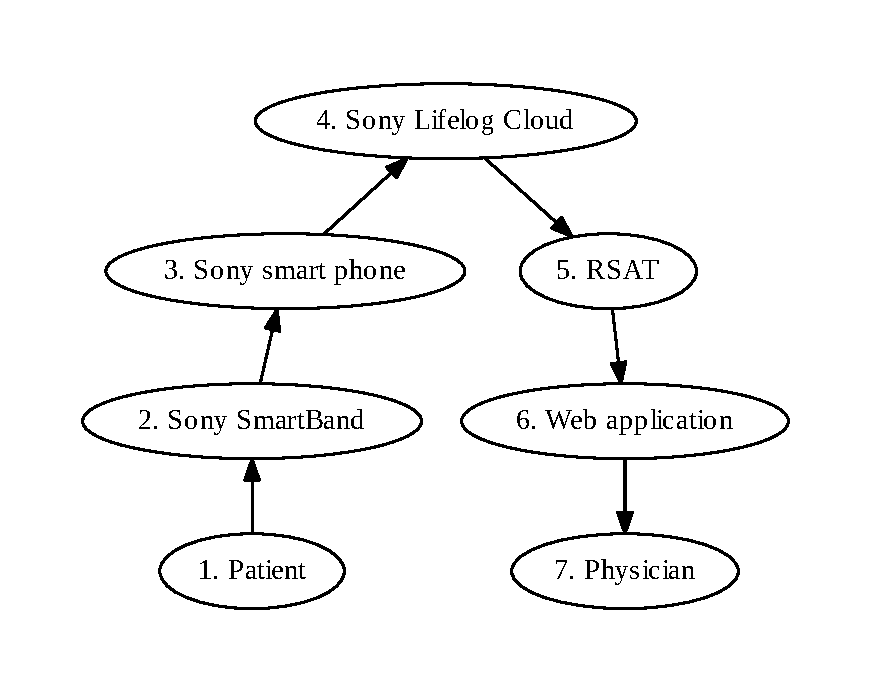
\includegraphics[scale=0.8]{proposed.pdf} 
\caption{Graph of the proposed solution}\label{fig:pro}
\end{figure}


\begin{enumerate}
    \item Each patient added in RSAT has a smart Sony SmartBand wristband around their wrist.
    \item The wristband collects data about the patient movements and the data is categorized into different activities.
    \item A Sony smartphone collects the data from the wristband via Bluetooth 4.0. 
    \item The data is stored in the Sony Lifelog application on the smartphone and synchronized with Sony's online service.
    \item RSAT fetches the data from the patient, analyzes it and saves it to a database.
\item The RSAT web application retrieves the data from all patients in the database and visualizes it to the nursing staff.
\item From the computer the nurse can interact with RSAT and see the progress of the patients. 
\end{enumerate}

\subsection{Process of adding a patient}

Each patient in the program needs an activity tracker and something to sync the data to the cloud with. Because of the use of SWR10 and limitations of lifelog to only track biking on SONY phones. It was decided to equip every patient with a SONY phone for syncing and SWR10. These phones and smart band was borrowed from the hospital. To make it easy for the nursing staff and the patients to get started each phone and smart band was preconfigured. The process for doing so was the following:

\begin{enumerate}
    \item{Phone and SmartBand is unboxed and charged.}
    \item{A new Google account is created for the phone.}
    \item{The Google account is used to download the apps:
\begin{itemize}
    \item Lifelog
    \item SmartBand SWR10
    \item SmartConnect 
\end{itemize}}
    \item{The Lifelog application is logged in to via the Google account.}
    \item{SmartBand is synchronized with the phone.}
    \item{The phone is added to our system and given a name.}
    \item{The phone and SmartBand is marked with the name of the phone and SmartBand inserted in the system.}
\end{enumerate}

So when the nursing staff give smart band and phone to the patient the only thing the nursing staff do is linking the patients profile to the phone in RSAT. %%Denna meningen är urusel 


\chapter{Development}
This chapter describes the development cycles of the RSAT. It also gives a brief introduction to the different 3rd-party libraries and palcom services that have been used to build the RSAT.

\section{3rd-party libraries and sevices}
This section gives a brief introduction to the different 3rd-party libraries and palcom services that have been used to build the RSAT.

\subsection{JavaScript libraries}
Several different JavaScript libraries have been used to develop the web application of RSAT. A short explanation of the different frameworks that have been used the most are given below:

\begin{itemize}
    \item \emph{Backbone.js} - Is a framework used to provide structure to web applications. It provides models, collections and views that can connect to existing API:s over a RESTful JSON interface\cite{osmani2013developing}. 
    \item \emph{Highcharts} - Is a library for making charts on the web using JavaScript\cite{kuan2012learning}.
    \item \emph{Moment.js} - Is a JavaScript library used to parse, validate, manipulate, and display dates in JavaScript\cite{moment}.
\end{itemize}

\subsection{Palcom services}
\subsubsection{The database service}%TODO the itachi-jidder texten är inte så bra. fixa... 
\label{sec:dbservice}
The itACiH-project has developed a generic database service that can be extended to be used for database tasks using Palcom. The database service has one \emph{in-command} and one \emph{out-command}. Each command to the database has 6 parameters. In this project only two of the parameters; json and classname are used: 

\begin{itemize}
    \item \emph{json} - This parameter describes the parameters sent to the database in a json format. 
    \item \emph{class-name} - This parameter tells the database service how to interpret the json-data sent in the json-parameter by providing the name of a predefined class in which the keys in the json-parameter exists as attributes.
\end{itemize}

Depending on what class-name that is stated in a command received in the service, different database operations are performed. What operations to be performed are predefined in the service. 

An example of a command sent to the database service is the following: 

\begin{verbatim}
{
'json' : '{"userId":3,"date":"2015-02-15T00:00:00","steps":30}',
'classname'	: 'databaseStep.RequestAddStepInterval'
}
\end{verbatim}  

When this command is received, the server converts the json-data in the command to a Java object of the class "RequestAddStepInterval", which exists in the package "databaseStep". After that the service communicates with the actual database and performs the actions that are defined in a predefined statement in the service. If the service should respond to the command, an out-command is created and sent. 

	
\subsubsection{The WebServer service}
\label{sec:webserver}

\begin{comment}
WEB SERVER ANTECKNINGAR.. saker vi kanske vill lägga till och ha med: 
The server handles asynchronous communications between the service and the 

definierar era servies
skriver lite js
kopplar upp. 
öppnar en socket. 
kommer upp som en device utan servicear
kan inte koppla ihop med assemblies
webappen måste veta vilka servicar den ska prata med
\end{comment}
The Palcom Web Bridge is used to connect web applications with PalCom services.  The PalCom Web Bridge is therefore referred to as the web server in this thesis. The first version of the web server was developed in 2012 and was based on long-polling and is described in the Palcom Web Bridge Design Document\cite{XXXXXXNULL}. The current version of the web server makes use of web sockets instead. 

To establish a connection between the web server and a service a configuration is needed. The configuration specifies deviceId, serviceId and instance. The configuration is used to establish a web socket. When the web-socket is established, in-commands can be sent to the service and out-commands can be listened to via the web service from a web-application.


\section{A proof of concept}

As a first step in the development, a proof-of-concept system was created. The proof-of-concept was developed to assure that data from several different users could be fetched from the Sony Lifelog API and viewed in a user interface. The system consisted of two parts, (1) a web application that served as the user interface and (2) a server that fetched the data from the API and handled the authorizations. The two parts of the system used HTTP for communication. To make the implementation of  the system as easy as possible, data about a user was stored to files. 

\begin{figure}[!hbt]
\centering
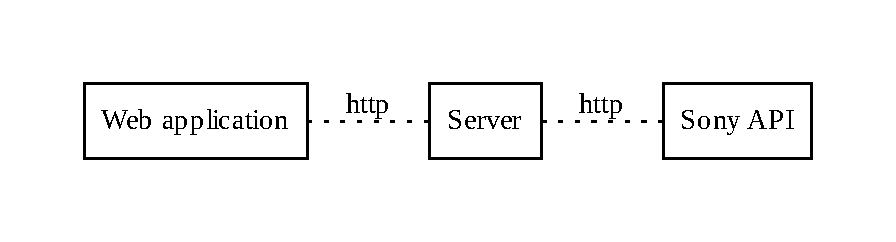
\includegraphics[scale=0.8]{firs_verison.pdf} 
\caption{An overview of the proof-of-concept system.}\label{fig:firstV}
\end{figure}

The web application was developed in JavaScript, using Backbone as framework. Figure \ref{fig:firstV_screen} shows a bar diagram that shows the number of steps user 15 has taken each day in a specific time interval. 

\begin{figure}[!hbt]
\centering
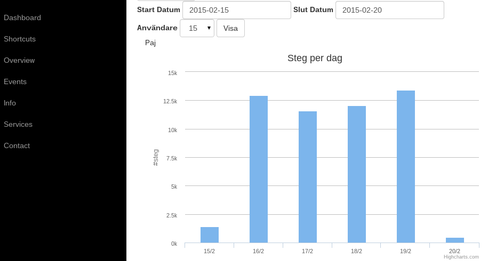
\includegraphics[scale=0.8]{first_prototype_screenshot_crop.png} 
\caption{A printscreen prototype 1}\label{fig:firstV_screen}
\end{figure}


\section{First iteration}
The foundation of the RSAT was created in the first iteration. PalCom was used to create services that was connected using assemblies. A description of the different services implemented and used in this iteration is given in the subsections of this section. 

An overview of the RSAT in the first iteration is shown in figure \ref{fig:second-version}.


\begin{figure}[!hbt]
\centering
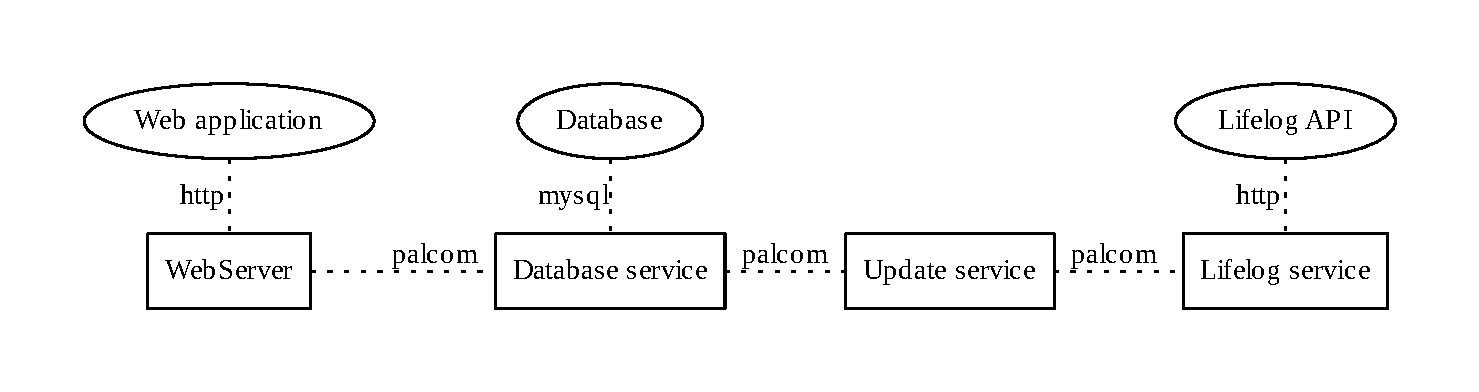
\includegraphics[scale=0.6]{second-version.pdf} 
\caption{An overview of the system in the first iteration}\label{fig:second-version}
\end{figure}

\subsection{The web application}

The web application is the user-interface to be used by the nursing staff. The nursing staff can view the data and goals for each patient in the RSAT from the interface. This part of the RSAT is written in JavaScript using Backbone as framework. When a nurse browses the activities of a patient the web application makes requests to the Database service through the web server. The communication between the web application and the web server is via HTTP.

\subsection{The web server} % todo: TO BE REWRITTEN! Jens tempos fråga

A generic web server is used for connecting PalCom services with the web application. The server handles asynchronous communications between the service and the web client. The web server is descibed in section \ref{sec:webserver}.


\subsection{The Database service}

The database handles the communications with the database. The database service is described in section \ref{sec:dbservice}. When it receives a command, it handles requests to the database and creates responses to be sent back to the service making the request and/or to other services. 


\subsection{The Update service}

The update service has the responsibility of periodically asking the Lifelog service for data from the Lifelog API and to send it to the Database service. The service requests data from the Lifelog service in a predefined time-interval. When the response from the Lifelog service arrives to the update service, the response is parsed and a command for adding the data in to the database is created and sent.


\subsection{The Lifelog service}

The Lifelog service is the gateway that connect the Sony Lifelog API to PalCom. The Lifelog API use OAuth 2.0 as its authorization mechanism. This means that the Lifelog service needs to obtain an access token for each user that gives permission to access the data in the API. 

The first time a patient is added to the RSAT, it must give permissions to the RSAT application to access it’s data in the Lifelog API. When the patient has given permission to the application, the application receives a response from the Lifelog API containing an access- and a refresh token. Since the access token is only valid for a short time-interval, the access token is not stored. Instead the refresh token is stored, which is valid for a unlimited time interval, or until the user revokes the access. 

When a Palcom command with a request for some data in the Lifelog API come to the Lifelog service. The service looks up the refresh token that belongs to that user in a database, and uses that token to request a new access token. The response from the API contains an access token and a new refresh token. The new refresh token is stored instead of the old in the database and the access token is used to access the Lifelog API. The response from the Lifelog API has a JSON format. This data is parsed and the interesting data is sent in a Palcom command. 

\section{Second iteration}

Additions made to the second iteration of the RSAT was to include more data types. The following data types was added to the system: 

\begin{itemize}
	\item Walking time
	\item Running time
	\item Biking time
	\item Calories burned
	\item Weight
\end{itemize}

Another feature that was implemented during this iteration was a feature such that it was easy to add new patients to the RSAT. In figure \ref{fig:second-itr} an overview of the RSAT from the second iteration is shown. The services implemented and improved in this iteration is described in the subsections below. 

\begin{figure}[!hbt]
\centering
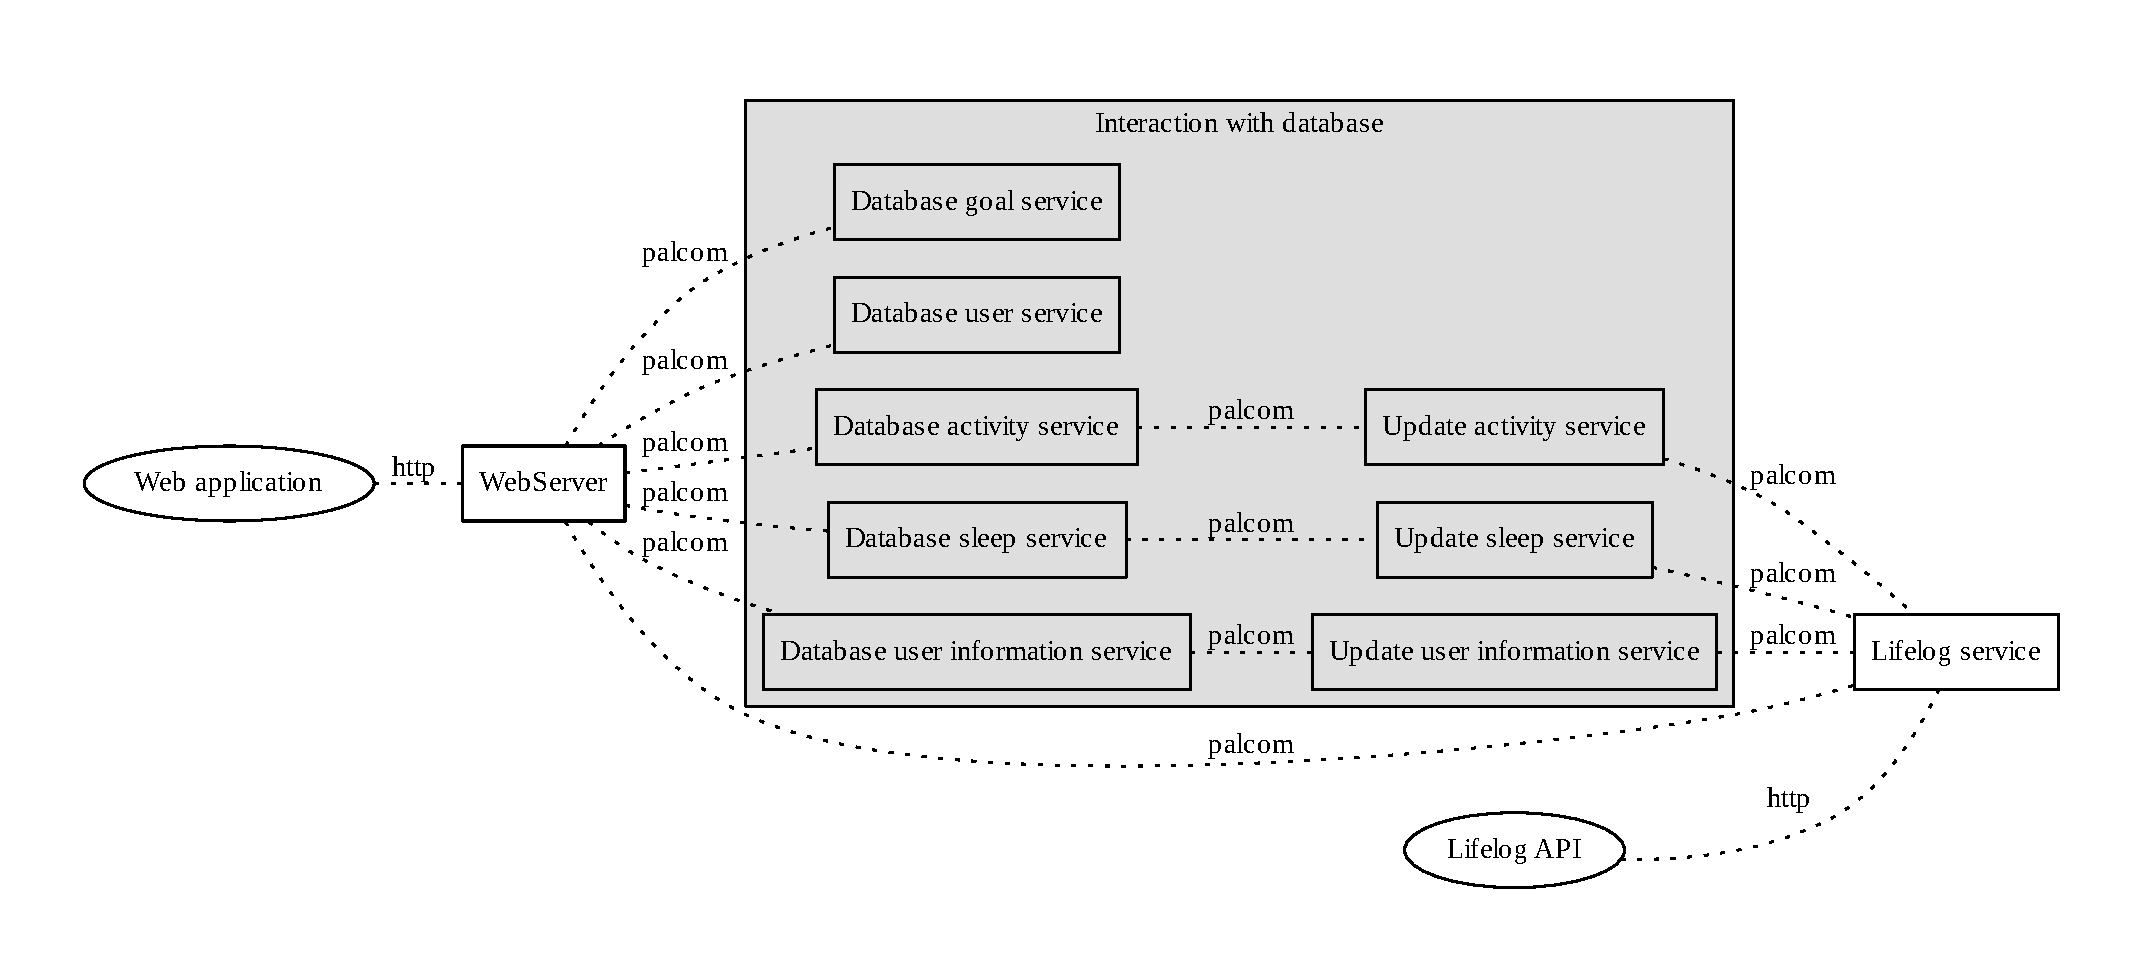
\includegraphics[scale=0.4]{forth-version.pdf} 
\caption{An overview of the system in the second iteration}\label{fig:second-itr}
\end{figure}


\subsection{Database services}

The generic database service was used to create different types of database services. The following database services was created: 

\begin{itemize}
\item \emph{The database goal service}, which are used to store all goals of a user. When the nursing staff inputs a goal for an activity in to RSAT this service save that goal to the database. The service also handles the fetching of these goals. %(TODO: skriva mer om) kolla jens.
\item \emph{The database user service}, which handles the the names of smartphones in the system by mapping the name on the phone to an ID number. %(Todo. förklara bättre) Jens läs. 
\item \emph{The database activity service}, which stores different activities and other data parsed from the Lifelog API. The data stored in the activities database service is parsed from the activities endpoint in the API. 
\item \emph{The database user information}, which stores personal information about the users. The data is parsed from the Lifelog API.
\item \emph{The database sleep service}, that stores information about a users sleep. The data is parsed from the activities endpoint in the Lifelog API.
\end{itemize}

\subsection{Updater services}
Updater services schedules and triggers the updates of users data in the database. In this iteration the updater service from iteration 1 has been divided up into several updater services. Each service has the responsibility of update a specific type of activity or a group of activities. The updater services fetches a list from the database with information about the users id’s such that it can query the Lifelog service for data. The task of updating the data of a user begins with the fetching of the date of the latest data point for the user. This date is sent to the Lifelog service such that the Lifelog service knows from when in time it shall start fetch data for the user. The service returns all data points from that user from the date returned from the database until current time. This datapoints are sent to the database service, which adds them to the database. 

The following database services exists in the RSAT:

\begin{itemize}
\item \emph{The Update activity service}, which triggers an update to update activity data.
\item \emph{The Update sleep service}, which triggers an update to update sleep data.
\item \emph{The Update user information service}, which triggers an update of user information.
\end{itemize}

\subsection{Adding users TO BE FIXED}

%(TODO Vi måste fixa med det här så att oauth-sker på rätt sätt. Eller förklara vad som inte är helt 100, KOlla jens) 

For adding a user to RSAT the first step is authentication of the user and getting the code. This code can then be sent to the Lifelog service for authorization of the Lifelog data.The authentication is done on Sonys authentication servers and the redirected back to the site with a code in the URL of the redirect. When making the redirect to the Lifelog authentication server, a state can be sent in the URL to the authentication server. This state is also in the redirect from the authentication server. In the solution proposed in this thesis a user name is provided before  the redirect to the authentication server. This user name is sent in the sate variable of the URL. After the redirection from the authentication server back to RSAT the user name is fetched from the URL and the user added to the system. The code from the authentication server is sent to the Lifelog service where the rest of the steps for authorization is done. This is not the correct use of the state parameter according to the OAuth 2 specification but there was no knowledge about this during the second iteration.

%todo Jag tycker vi tar bort det här kapitlet men det beror på vad du tycker. I annat fall är här en förkortning och stavrättad del jag tänker vi kanske kan använda: 
% In the Lifelog application, the user can input his/her current weight. This data is fetched from the application at a regular interval in the RSAT.  

%\subsection{Dealing with weight}
%Sony lifelong do not deal with weight over time. But it is possible to set the weight in the mobile lifelong application and the read the weight from the Lifelog API. To support weight over time RSAT fetch the weight for a user from the Lifelog API at regular interval. The weight is the added to the database together with the current date and time. Using this the RSAT system is able to build a history of weights over time.



\subsection{User interface}

In the second iteration of the RSAT, two improvements of the user interface was made:

\begin{itemize}
\item The views in the graphs was fixed such that the data shown was showed for one week at the time. 
\item The ability to change an activity goal at the same place as the data was shown for the activity was added.
\end{itemize}

These improvements was based on feedback from the project group. Figure\ref{fig:second-screen} shows the interface from iteration 2.


%TODO Detta kan nog användas för att bättre beskriva authentiseringen och de fel/genvägar vi gör när vi autentiserar en patient. 
%Most of the logic for adding a user is the in the web application. We have implemented a way to add users. To add a user a name is written in a form and a bottom pressed. The user is redirected to Sony's log in for authorization for lifelong API. In the redirect a parameter is sent to the url with the user name. This parameter is the 

% Name of system


\begin{figure}[!hbt]
\centering
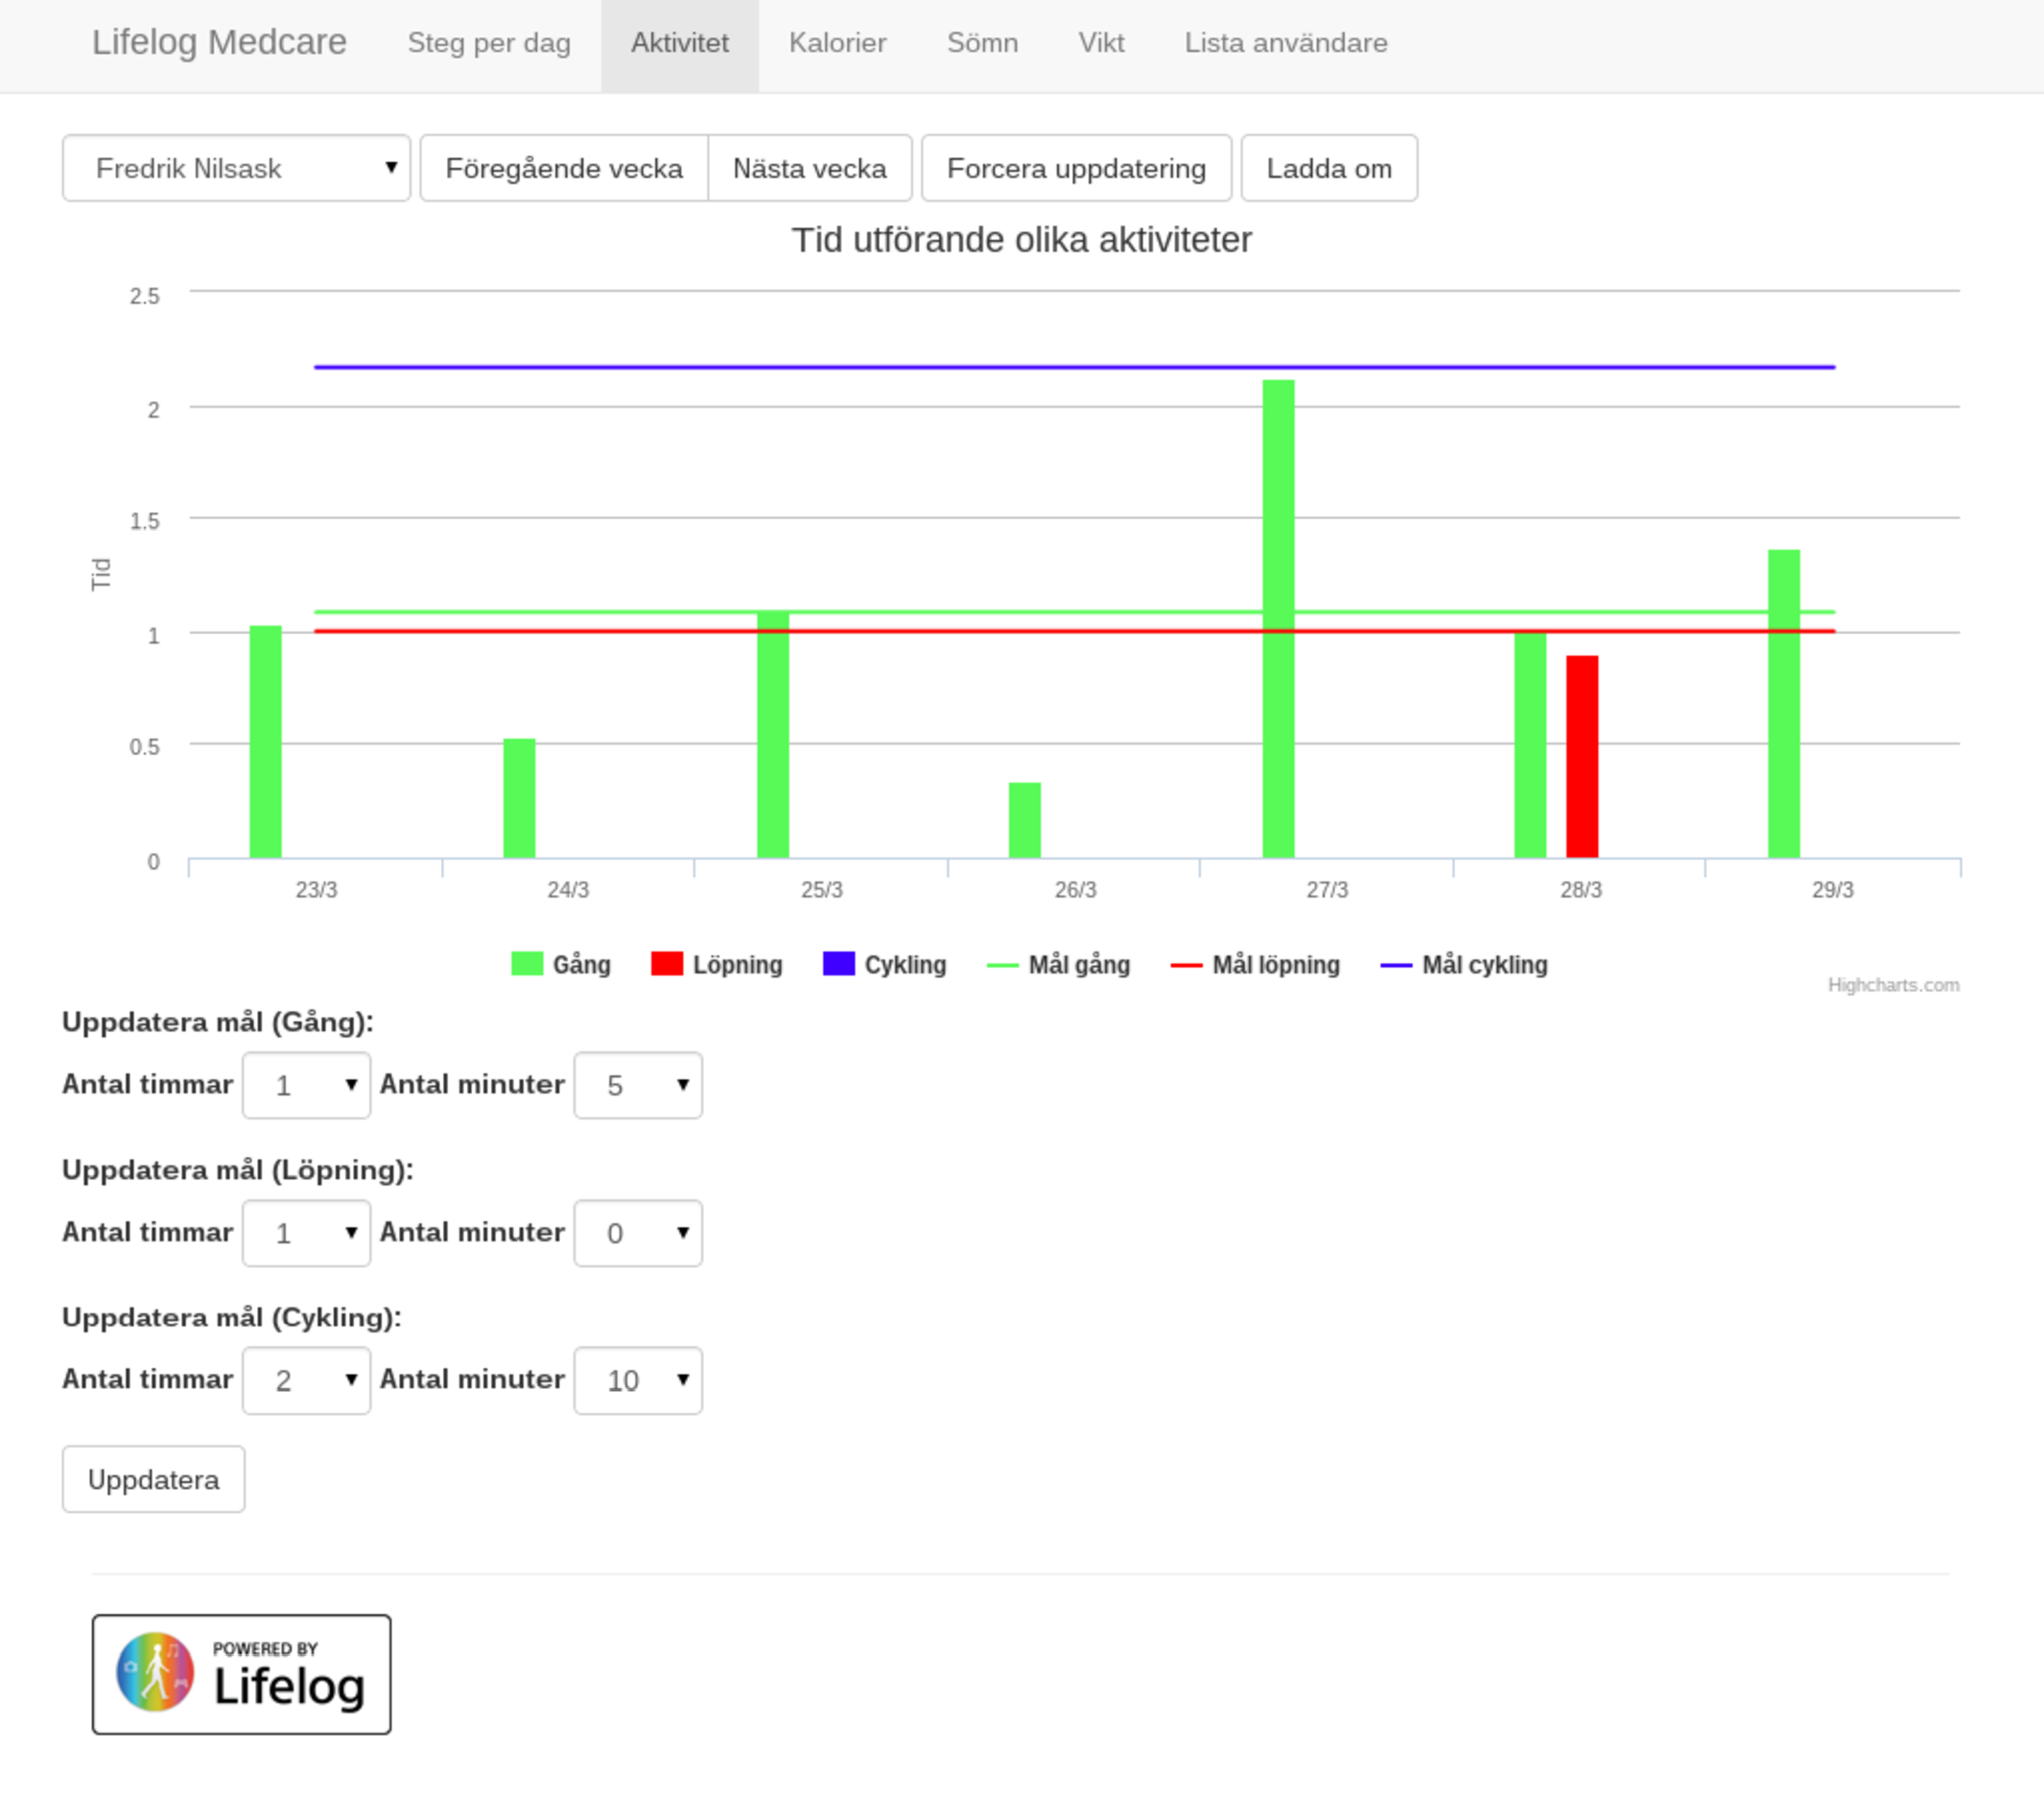
\includegraphics[scale=0.4]{seceenshot-second-version.pdf} 
\caption{Printscreen from the second iteration}\label{fig:second-screen}
\end{figure}

\chapter{Evaluation}
 This chapter presents an evaluation of both the Lifelog platform and the RSAT system. First the SWR10 is evaluated compared to the current market. Then API is evaluated on the basis of the RESTful practises and data consistency between app and API. The last evaluation of lifelog is done by comparing it to other platforms. In the second part of the chapter RSAT is evaluated by comparing is similar systems and the fulfillment of the requirement stated in section \ref{sec:req}. 

\section{Evaluation of the Lifelog platform}
\label{sec:utLifelog}

\subsection{The wristband to be used}
SWR10 is the wristband that initially will be used by the patients that are participating in the pilot program of RSAT. SWR10 has an accelerometer which is responsible of collecting all the different data the wristband tracks about a user’s activities.
%It would be interesting to know how accurate the gathered data actually is but no such information is available. Neither does it exist any information about what algorithms that have been used to process the data and to categorize it into different activities.
To get accurate data from activity trackers there are essentially two important things: (1) - to get good sensor data and (2) - good algorithms to analyze the sensor data. Studies about the quality of the sensor data and the algorithms for swr10 has not been found in the research process of this thesis.   

There exists other wristbands on the market that have more sensors. More sensors could imply that more accurate data could be collected. This however, is something that highly depends on the accuracy of the sensor data and the algorithms used. It is very important that the patients and the physiotherapist can trust the data that is gathered by the wristband to be able to draw concussions. More sensors should therefore not be included if there is a risk that the data collected i inaccurate. More sensors would not only mean that it was possible to collect more data, it would also mean that calculations about things such as physical activity could be improved since more data could be used as input to the calculations. 

The heart rate is something the physiotherapist has expressed an interest of being able to see. If the heart rate was known, it would be easier to know how active each patient is during a day. The fact that the SWR10 does not have any heart rate sensor is therefore one of its major disadvantages. On the other hand, it is good that Sony has chosen to not integrate a sensor that can not deliver useful data. As stated before, optical heart rate sensors tends to perform badly at higher heart rates. The usefulness of optical heart rate monitors when excercising are therefore somewhat debatable. But the data from a heart rate monitor could still be used as input to find out wether somebody performs any physical activity or is inactive. This would be valuable information for the physiotherapist.

%Given that the sensors that are used can fetch data that is accurate and that the algorithms used to process the data are adjusted to take the data into account, more sensors would be preferable. 


To compare the results of different wristbands and tell which one that is the most accurate an empirical investigation would be needed.  


Some of the smart bands has display and this makes the smart band more independent of the phone. When the display shows the progress the only use of the phone is the sync the data to the cloud. In our case real time update is not an important feature so syncing the band once a day would be acceptable. Therefore a display could eliminate the need for patients to walk around with a phone all the time.

%For patients to be able to use the smart band independent, without the use of an phone. A screen is important to be able to see the progress of training. Here the swr10 has drawbacks but sony has an swr30 with a screen. 

Mer text kommer här...

\subsection{The Lifelog API}

The Lifelog API will be evaluated from two different perspectives. (1) - Is it a rest API? If it is a REST-API it follows the same standards as most modern web-API:s and should therefore be considered to be easy to use. (2) - Is the data that the API contains consistent with the app? 

%Jag tror att de här frågorna behöver fixas till lite. Det är inte riktigt det som är tanken... Men vi vill nog utvärdera något mer än ifall det bara är ett REST-api eller inte. Har du någon bra idé Alfred? Allt är inte tillgängligt. Tillexempel mål. Det borde också framgå... Vi får hitta på lite bra rubriker här... 
%Evaluation of the results have been based on comments and facts provided by the nursing staff at the Skåne University Hospital. It has also been based on comparison with other similar systems on the market. 


%todo api är readonliy
%todo api visar inte all data. tex goals. 

\subsubsection{REST or not}

Sony states that the Lifelog API is REST-based. In order to be a REST-API the API must fulfill the architectural principles that was presented in chapter \ref{sec:rest}. We have evaluated the API and concluded that it actually is a REST-API. Below you find comments on why the API fulfills each principle: 

\begin{itemize}
    \item \emph{Addressability} - Each request to the Sony Lifelog contains a time-interval and a list of datatypes telling what you want your response to contain. No matter when or how many times you query the API, you will query for the same data. The addressability principle therefore holds, as you can address a resource using a unique URL. 
    \item \emph{Uniform interface} - The Sony Lifelog is a read-only API and only supporting GET requests. It therefore has a uniform interface.
    \item \emph{Stateless Interaction} - The communication with the API is stateless. The only exception to this is the authentication part of the communication, that is using OAuth2. When an access token is issued, the the API must verify that the client's credentials is correct and the authentication is therefore not stateless. However, the authentication can be seen as something that happens before the connection to the API which would make the API-communication completely stateless. 
    \item \emph{Self-describing Messages} - The strings used to query the API are self-describing and uses distinct parameters. The responses have a JSON-syntax are also self-describing and have distinct parameters. 
    \item \emph{Hypermedia} - The hypermedia principle is used by the API when the requested data is too large to fit in a single response. The API uses links that it sends with the first part of the response. These links contains the url to the rest of the queried data.

\end{itemize}

\subsubsection{Lifelog Application compared to Lifelog API}
There are two things in the Lifelog application that is missing in the API. First, goals the user set in the app can not be read from the API. Second, in the Lifelog app the user can bookmark different moment. These moment can neither be read from the API. Activity and profile data on the other hand can easily be read from the API. An when steps per day for example was calculated using the data form the API it was the same the calculation done in the app. But no data can be written to the API.

\subsection{Lifelog compare to other activity tracking platforms}

\subsubsection{Lifelog compared to Google fit}
Google Fit and Lifelog both has a REST API that third party users can use to fetch activity data. It is possible to write data to the Google Fit API, something that is not possible in the Lifelog API. This makes it possible to integrate data from sensors manufactured by different companies in the API. Both Google and Sony provides a uniform interface for different activity trackers. Although the Lifelog API only contains data from Sony products, all their different products collects data that has the same structure in the API. Google has clearly stated that their API is not to be used in the health care. This means that Google fit is not appropriate to be used in RSAT. But besides that, Google Fit has a lot of attributes that would make it useful in RSAT. It has all the capabilities that Lifelog has and also makes it possible to import data from other sensors into the API. 



\subsubsection{Lifelog compared to Apple health} 

The big difference between Apple Health and Sony Lifelog is that Apple Health does not have a cloud API. Apple, on the other hand, has an API that applications run on their phones can use to insert and fetch data. Since the Sony API is read-only, it is not possible to insert any data at all for third-party users, a major disadvantage in comparison to Apple Health. 

\subsubsection{Lifelog compared to Jawbone UP Platform}

The UP platform is more open than the Lifelog platform. The cloud api is both writable and readable. They also provide a low level API that different Bluetooth devices can use to write data to the platform. The Bluethooth API gives sensor manufacture the possibly create a sensor without the need for a companion application. This functionality lack the Lifelog platform.   


%\subsection{Summary}
%In this summary we summarize bla bla bla. 

\section{Evaluation of RSAT}

In order to evaluate RSAT we need to compare it with other similar systems on the market. In this section a comparison with Tactio and Fruit Street will therefore be performed. It will also be compared to wellness programs that has a similar functionality but another use case. 
%... bla bla bla

\subsection{RSAT compared to Tactio}

Tactio has developed a smartphone application that is to be used by each patient. This is a fundamental difference between Tactio and RSAT. The application makes it possible for Tactio to customize each patient’s experience. We have found three major advantages with this approach. (1) - Tactio can decide by them self what data that shall be shown in the application. This means that data they consider to be irrelevant in the manufacturer’s application can be ignored. (2) - It makes it possible for Tactio to fetch data from sensors from several different manufacturers and to visualize the fetched data for the patient in a uniform way. This data can also be used as input to algorithms that can create new more accurate data. (3) - Custom made feedback- and notification messages can be generated and sent to the applications from the clinicians. Different kinds of activity goals can also be generated by the clinicians and visualized in the application. The only disadvantage with their solution is that they have to invest a lot of resources in order to create their application such that it can deliver a good user-experience for the patients. Since most manufacturers already have created an application Tactio must create an application that is equally good or better in order to get the patients to use theirs instead. 

RSAT periodically downloads data from the Lifelog API and saves it on a server inside the hospital, where it is not accessible from the outside. Tactio saves the data in their own cloud and is made accesible through an API. This API can be accessed to fetch data into other hospital systems. RSAT have no API which can be queried from the outside of the hospital network. However, it is something that would be easy to add support for in the future if needed.  

The  clinicians using the Tactio system can only interact with the patients via an iPad application. RSAT is built as a web application and can be accessed through any web browser meaning that it can be accessed through any web browser. This is both an advantage and a disadvantage at the same time. The advantage is that the clinicians only need to learn one platform and that the application will always have the exact same structure. The disadvantage is that it only can be accessed from an iPad.


\subsection{RSAT compared to Fruit street}

Patients that are participating in the program where RSAT is to be used borrows a pre-configured smartphone and wristband from the health care. In Fruit Street, each patient connects their own fitness tracker. This is a significant difference between these two systems. In fruit street the patient has to follow a multiple stage process to add their wristband to fruit street  while in RSAT everything is configured and ready to go when the patient get their wristband and smartphone. 

Fruit Street is more flexible in regards to how goals can be created for each patient. The only type of goal that is possible to create in RSAT is daily goals, where in Fruit Street a goal can have an arbitrary length, meaning that you can create a monthly or weekly goal. 


\subsection{RSAT compared to Wellness programs}
What RSAT and the wellness programs described in chapter \ref{sec:wellness-programs} have in common is the ability to monitor peoples activity using activity trackers and to visualize the data in a common dashboard. 

Smart wear manufacturers that are creating their own wellness programs have have full control over both hardware and software. This means that they can customize the hardware and software as they want when implementing a feature. It also has the advantage that they can make use of functionality that does not exist in their public API:s. Garmin has taken advantage of this by creating the Vivohub. This eliminates the need that every employee must have a smartphone in order to synchronize their data with the wellness program. The disadvantage with such a system is that a company that chooses to use a wellness program developed by a manufacturer can not integrate other sensors from other manufacturers. 

\subsection{Fulfillment of requirements}

In this section all requirement are gone thought and seen if they are fulfilled. All wanted types of activity data from lifelog were implemented in RSAT. By using diagrams it was also possible to show the history of the data. The requirement of the user interface to be easy to use is hard to verify but a popular UI library were used to make it look familiar for web-users. It is also easy to create goals for every patient each every data type,. Because the patient has the same goals in the lifelog app as in RSAT it is possible to view the goals. A problem with this is that the patient and the nursing staff must sit together to set the goals. The requirement for measurements of inactivity was not fulfilled. Because the possibility to get activity data in real time was limited and required the smart band to always be connected to the phone. It was decided to not implement this feature.  An overview of the patients and whether they have completed their goals was not implemented due to a lack of time. But an detailed view for ever patient was implemented. To add another wristband only one service with the same commands as the Lifelog service has to be written. The authentication of this new has to be taken into account and added to the web-application. 




% TODO (Fixat läs jens) possibility to add other wristbands to the system? Borde vi diskutera det någonstans. Kanske i prestudy.

%\subsection{Summary}

Lägg i dicussion. 

%A limitation of the system is that the goals has to both be set in the app and the web application. There are two possible solutions for this problem. One is the possibility of writhing an app for the patient to use and that way to set goals. The other possibility is for the lifelog api to change for allowing goals to be read and writhed.

%The downside with this solution is that the Lifelog API is a readonly API. This means that it is not possible to send custom made feedback messages to the patients since they are using the Lifelog application. 



\begin{comment}
\subsection{Användbar data}
\begin{itemize}
	\item  utgå från RSAT och dess pilot
	\item  gör en empirisk undersökning där Mia svarar
	\item  todo: göra en enkät. 
\end{itemize}

\subsection{Funktionalitet som inte finns men som man vill ha}
\begin{itemize}
	\item utgå från Mia
	\item utgå från de andra systemen
	\item utgå från önskemål och tankar från adnra i projektgruppen
\end{itemize}

\subsection{Problem med API:t från en teknisk jidderasdasdasd}
\begin{itemize}
	\item kolla om det är ett REST-api?
	\item Reliability? 
	\item bra att de följer standarder. 
	\item API:et begränsar plattformarna. bara Android/Sony
	\item Tekniska problem vi har inte kontroll över datan. 
	\item Vi måste anpassa applikationen efter deras data
	\item bättre om datan kunde hämtas direkt utan att synkas upp i molnet. 
	\item 
\end{itemize}


\begin{itemize}
\item jämföra vårt system med befintliga
\item saker som fattas i sonys aktivitetsband, saker som finns i andra som vi hade velat ha. 
\item Jämför Sony Lifelog plattformen med de andra plattformarna. 
\item bygga eget ekosystem eller plugga in datan i tex google fit? 

\end{itemize}
\end{comment}


\chapter{Discussion}

\chapter{Conclusions}

\section{Future work}
   
\makebibliography{bibliography}

\end{document}

\begin{comment}
\chapter{Approach}

%% Skriva ner totala målet osv... Kravspec på systemet... 


\section{First project plan}
We, Jens and Alfred sat down with one of our advisers Fredrik. He had make an proposal for a timetable and we where together collaborate and made it more reasonable. This is the first version of the time timetable. The timetable is divided in to four different parts, around 1 month each.

\subsection{Part one}
From mid February to mid March.

\begin{itemize}
\item A standalone system the can be reach from the internet with a interface that is easy to use.
\item Be able to see steps and sleep for a group of patients, including the possibility of setting goals.
\item The people testing in the part is Mia, Fredrik , Jens and Alfred. 
\end{itemize}

\subsection{Part two}
From mid March to mid April.
\begin{itemize}
\item Authorization should be atomized using for example a android app. 
\item The system should be able present walking time, running time, biking time, inactivity time and number of calories including the possibility of setting goals.
\item The people testing in the part is Mia, Fredrik, Jens, Alfred, Bosse and the team.
\end{itemize}


\subsection{Part three}
From mid April to mid May.
\begin{itemize}
\item Integration with the itACiH system.
\item Target achievement appear in the list of patients.
\item Reminder of long inactivity
\item In the test group is Mia, Fredrik, Jens, Alfred, Bosse, the team and selected patients.
\end{itemize}

\subsection{Part four}
From mid May to mid June.

\begin{itemize}
\item The master thesis end.
\item The pilot study run for some more time.
\item Bravo message when goals are accomplished if time allows.
\item More custom goal if time allows.
\item Sharp testing with real patients.
\end{itemize}


\end{comment}